\chapter{Introducción}
\noindent Para el desarrollo de software se debe considera aspectos que influyen en el precio que debe pagar el usuario final como ser: Costo de desarrollar el software, Costo de mantenimiento, Costo del entorno de ejecución,  Costo por agregar nuevas características, el número de usuarios a utilizar el software, y el modelo de distribución que define como es que el usuario final va adquirir el producto y las nuevas versiones. 

\section{Descripción del problema}
\noindent En el negocio de desarrollo de software de propósito general o comercial, los costos de desarrollo, mantenimiento, tener  entornos de ejecución (servidor) por el lado del cliente y la distribución del producto son determinantes para definir el precio que el usuario pagara por el producto.

\noindent A continuación se describe situaciones que afectan el incremento del precio del software:

\begin{itemize}
   	\item Instalación y actualización del software en diferentes lugares geográficos, lo cual hace que el proveedor tenga un soporte técnico para la puesta en ejecución y 	 las respectivas actualizaciones del software en los ambientes de ejecución de los clientes. Por otro lado los clientes que pueden ser empresas necesitan tener un departamento de Tecnología e Información que administre los ambientes de ejecución, agregando recursos de hardware a medida que pueda ir necesitando el software.
    \item Los clientes no siempre pueden llegar a tener la última actualización, algunos podrían estar trabajando con versiones anterior y esto hace que el proveedor tenga que dar soporte técnico a estas versiones.
    \item Agregar nuevas características al software también puede ser un factor determinante en cuanto al tiempo y costo que puede tomar.

\end{itemize}

\noindent Actualmente el desarrollo de software está siendo enfocado a ofrecer servicios en la nube (internet) donde usuarios potenciales puedan usar el software sin la necesidad de instalar en sus equipos. Esta manera de que el usuario final pueda acceder y utilizar el software, se lo denomina “Software como un servicio – Software as a Service (Saas)”, El cual es un modelo de distribución de software.

\section{Objetivos}
\noindent En este proyecto de grado, se pretende alcanzar los siguientes objetivos:

\subsection{Objetivo General}

\noindent Implementar un Software como un servicio, optimizando los recursos en el proceso de desarrollo del software. 


\subsection{Objetivos Específicos}

\noindent Para lograr el objetivo General, se pretende realizar los siguientes objetivos específicos:
\begin{itemize}
  \item Aplicar la metodología 12factor en las diferentes etapas de AUP, para el desarrollo de un Software como un Servicio – SaaS.
  \item Hacer uso de un servicio en la nube que proporcione  infraestructura en hardware y software para los entornos de ejecución. De tal forma que se puede aumentar o disminuir los recursos de acuerdo a la demanda (número de clientes que usan el software).
  \item Implementar un modelo que defina, la automatización de instalación de ambientes de desarrollo, construcción de ejecutable, verificación de los cambios nuevos en el código no afecte a funcionalidades ya definidas anteriormente, y la puesta en ejecución de la aplicación.
\end{itemize}

\section{Justificación}
\noindent En este proyecto de grado se pretende justificar en los siguientes ámbitos:
\begin{itemize}
  \item \textbf{Metodológico:} Se pretende plantear un modelo para optimizar el proceso de desarrollo hasta la puesta en ejecución de la aplicación. Considerando aspecto de: versionamiento de código, automatizar la preparación de entornos de desarrollo y ejecución e Integración continua.
  \item \textbf{Social}: Una guía para estudiantes o profesionales que se están introduciendo o se dedican al desarrollo de software. Como caso de estudio, se ha considerado realizar una aplicación web para la administración de pedidos en mototaxis que sera de mucha ayuda para las empresas dedicadas en  éste rubro.
  \item \textbf{Tecnología}: Como plataforma principal se pretende usar Nodejs que define una arquitectura manejado por eventos – Event Driven lo cual permite crear aplicaciones escalables.
\end{itemize}

\section{Limites y Alcances}
\noindent En el proyecto de grado se pretende enfocar más al proceso de desarrollo del software y la puesta en ejecución. Para lo cual se define los siguientes límites y alcances:
\begin{itemize}
  \item No se realizara un estudio de costo. Se realizara un enfoque más a los factores que pueden afectar al costo de producto.
  \item Los factores que se consideraran: desarrollo del software, distribución, ambientes de ejecución, y el mantenimiento.
  \item Para los ambientes de ejecución, se utilizara servicios en la nube como ser heroku o docker. De tal forma que no sea necesario instalar o preparar un servidor.
  \item En el caso de estudio. El software como un servicio será estándar para todas las empresas del mismo rubro. Lo que significa que no se podrá extender o agregar nuevos complementos para personalizar en las diferentes empresas.
\end{itemize}

\section{Diseño metodológico}
\noindent La metodología 12factor definida por [Adam Wiggins, 2012], está enfocada para el desarrollo de aplicaciones SaaS (Software as a Service). Esta metodología trata de que en el proceso de desarrollo del software se cumpla ciertos objetivos, los cuales son:

\begin{itemize}
  \item Tener una configuración automatizada para los entornos de desarrollo, puesta en ejecución de la aplicación.
  \item La aplicación debe ser portable entre los diferentes entornos de ejecución.
  \item Tener un conjunto de herramientas para la puesta en ejecución de la aplicación en plataformas en la nube.
  \item La aplicación debe ser escalable de tal forma que se realicen mínimos cambios de herramientas, arquitectura, o prácticas de desarrollo.
\end{itemize}

\noindent Para lograr los objetivos citados anteriormente, la metodología 12factor se enfoca en los siguientes puntos: 
\begin{itemize}
  \item Código base: Versionamiento de codigo en un repositorio central.
  \item Dependencias: Explícitamente declarar y aislar dependencias.
  \item Configuración: La informacion de conexion a base de datos, servicios externos, credenciales, configuracion de entornos de ejecucion. 
  \item Servicios externos que utiliza la aplicación: tener los servicios externos como recursos adjuntos que pueden ser cambiados en cualquier momento.
  \item Construcción, lanzamiento, y puesta en ejecución: Tener las etapas de construccion, lanzamiento y puesta en ejecucion independientemente. 
  \item Procesos: Poder ejecutar la aplicacion en un o mas procesos. 
  \item Enlazamiento a puerto: los servicios de la aplicacion deben estar expuesto atraves de un puerto.
  \item Concurrencia: Definir un modelo arquitectonico que soporte escalabilidad
  \item Minimizar el tiempo de inicio y apagado de la aplicacion: Despliegue rapido de codigo o cambios de configuracion y la puesta en ejecucion en los ambientes de produccion.
  \item Paridad entre los ambientes de desarrollo y producción: despliegue de cambios de un ambiente a otro sea ripido, al momento de trabajar en arreglar error o problemas que se dieron en produccion.
  \item Registro de eventos. Logs: Nos permite tener un registro de lo sucedido cuando se presenta un problema de la aplicacion que esta disponible para los usuarios.
  \item Administración de procesos: para incrementar las instancias de la aplicacion dependiendo a la frecuencia de usuarios esten usando la aplicacion al mismo tiempo, Proceso de migracion de bases de datos, ejecucion de script para la validacion de cambios en el codigo fuente.
\end{itemize}

\noindent La metodología AUP se enfoca en el desarrollo de aplicaciones usando técnicas agiles como ser Desarrollo dirigido por pruebas,  Modelo Ágil, Gestión de Cambios Ágil.

\noindent La metodología AUP define las siguientes etapas:

\begin{itemize}
  \item \textit{Inicialización:} Identificación del alcance del proyecto, definir una potencial arquitectura.
  \item \textit{Elaboración:} Proveer una arquitectura más clara del software.
  \item \textit{Construcción:} Implementación del software basados en las características de prioridad alta para los inversionistas. 
  \item \textit{Transición:} La validación de software y la puesta en ejecución en los ambientes de producción.
\end{itemize}

\noindent Principios de la metodología AUP:
\begin{itemize}
  \item \textit{Modelo:} Comprensión de las reglas de negocio, plantear diseños de solución para los problemas de dominio.
  \item \textit{Implementación:} transformar los modelos, diseños en código y ejecutar un básico nivel de pruebas (pruebas de unidad).
  \item \textit{Pruebas:} Realización de evaluaciones para asegurar la calidad del producto.
  \item \textit{Puesta en ejecución:} desplegar el software en los ambientes de producción y que esté disponible para los usuarios finales.
  \item \textit{Administración de configuración:} Administración de los artefactos del proyecto y versiones.
  \item \textit{Administración del Proyecto:} manejo de riesgos, direccionamiento de personas.
  \item \textit{Entorno:} se enfoca en las necesidades del equipo de desarrollo, que se está siguiendo el proceso (estándares y guías), herramientas (hardware, software, etc.).
\end{itemize}

\begin{figure}[ht]
  \centering
  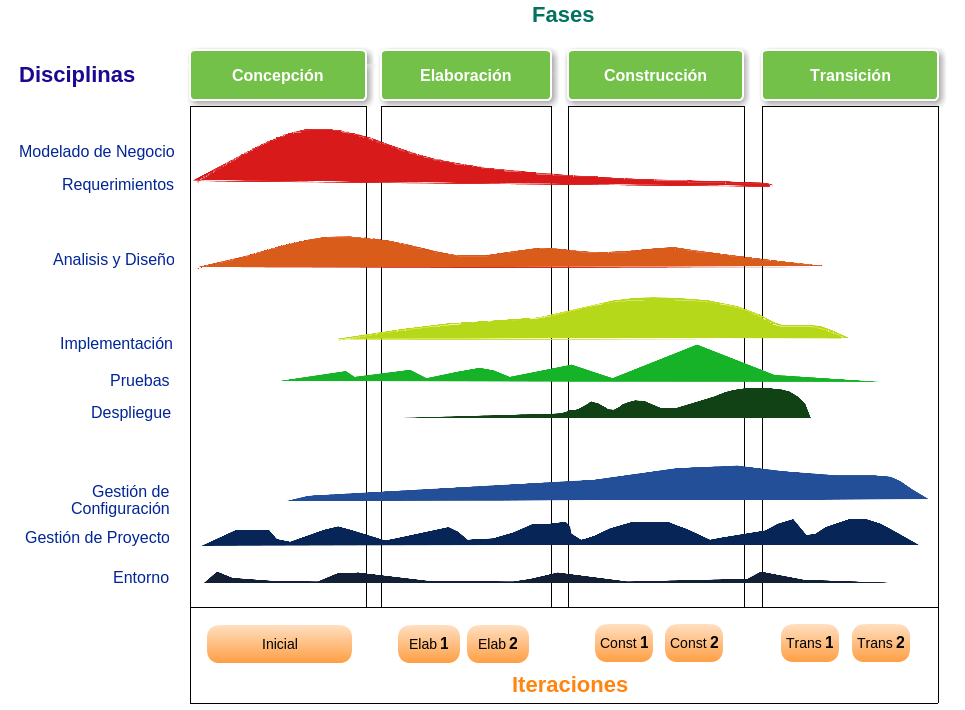
\includegraphics[width=15cm, height=9cm]{chapter1-aup-stages.png}
  \caption{Aplicación de las disciplinas en las fases del Proceso Unificado Agil AUP [Elaboracion propia ]}  
\end{figure}

\begin{figure}[ht]
  \centering
  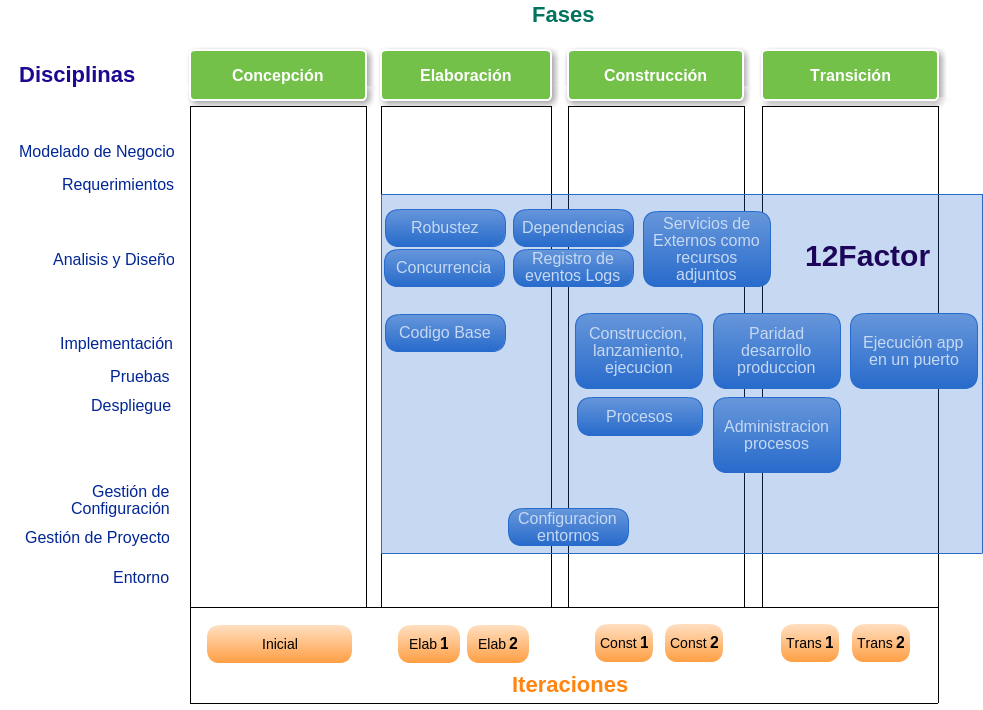
\includegraphics[width=15cm, height=9cm]{chapter1-model-12factor-aup.png}
  \caption{12factor introducida en las disciplinas de AUP en las diferentes fases (Elaboración propia)}  
\end{figure}

\begin{figure}[ht]
  \centering
  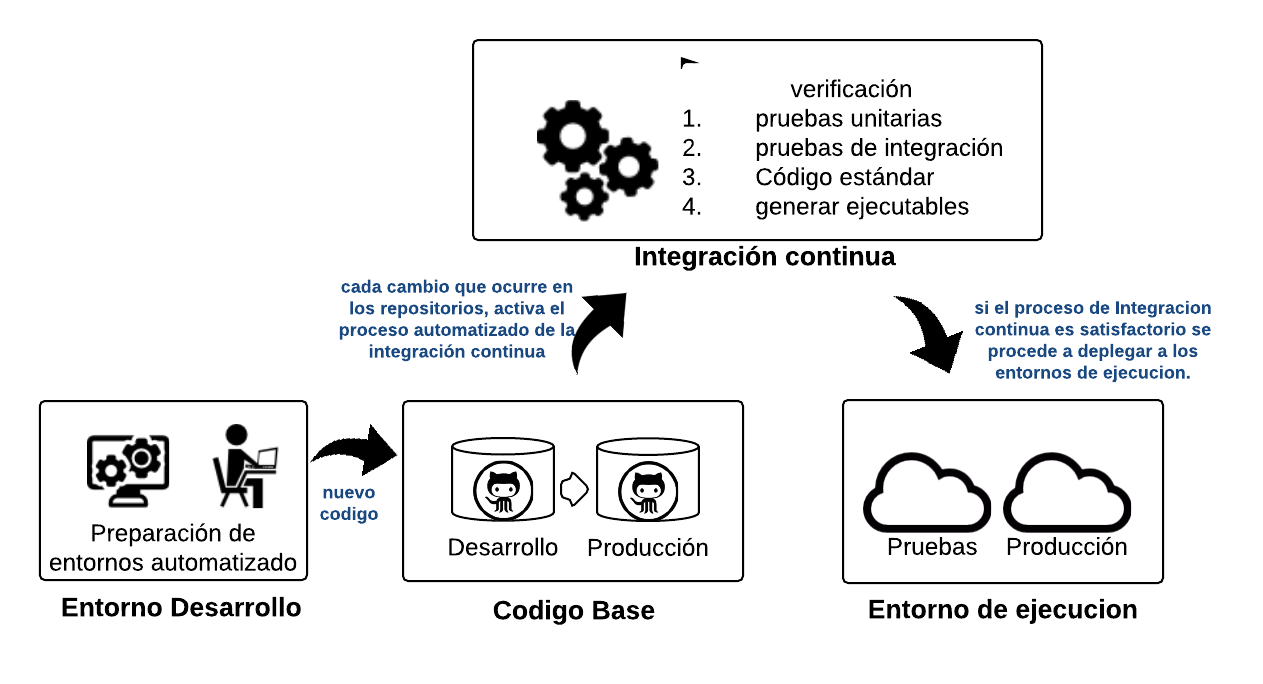
\includegraphics[width=12cm, height=6cm]{chapter1-model-process-development.png}
  \caption{Automatización de procesos, desde la preparación de ambientes de desarrollo, validacion de cambios en el codigo base y despliegue de los cambios en los ambientes de ejecucion (Elaboración propia)}  
\end{figure}
\noindent Tener tareas automatizadas en el proceso de desarrollo del software como ser: preparación de entornos de desarrollo para nuevos desarrolladores, validación de nuevas caracteristicas o arreglo de errores, introducida al codigo base. Verificando si se esta siguiendo el codigo estandard definida por el equipo de desarrollo, ejecución de test unitarios y de integracion, generacion de ejecutables y la puesta en ejecucion. Aceleran el proceso desarrollo del software y aseguran que los cambios introduciodos al codigo base, sean de incremento de tal forma que las nuevas caracteristicas no afecten a las anteriores.




